% chapter 08 - yuze
\documentclass[../main.tex]{subfiles}

\begin{document}

\section{Geometrically attracting and repelling fixed points}
\label{sec:8}

As discussed in the introduction, the value of the \emph{multiplier} $\lambda$ is of crucial importance in determining the local behaviour of the function. This section will mostly be concerned with the case $\abs{\lambda} \notin \{0, 1\}$. Specifically, we study
\begin{enumerate}
    \item $0<\abs{\lambda}<1$ corresponding to \emph{geometric attraction}, and
    \item $\abs{\lambda}>1$ corresponding to \emph{repelling}
\end{enumerate}.
As before, we study a holomorphic map $f:\nhd \to \C$ that is analytic in a neighbourhood $\nhd \subseteq \C$ of the origin which is a fixed point

\begin{equation}
    \label{8:eq:f}
    f(z)=\lambda z+a_{2} z^{2}+a_{3} z^{3}+\dots
\end{equation}

\subsection{Attracting Fixed Points}
\label{8:sec:att}

\begin{dfn}
    \label{8:def:att}
    The fixed point $\fix$ of $f$ is called \emph{topologically attracting} if\, $\exists$\, a neighbourhood $U$ on which the iterates $\iter{f}{n}$ are defined and converge uniformly to the constant map $z \mapsto \fix$.
\end{dfn}

\begin{rmk}
    \label{8:rmk:uniffix}
    It is important that we demand the convergence to be uniform. Intuitively, this is because we want to imply the notion of a neighbourhood that ``shrinks'' under iterations of $f$ to an arbitrarily small size.
\end{rmk}

\begin{lem}[Topological Characterization of Attracting Points]
    \label{8:lem:att}
    With $f$ as in \eqref{8:eq:f}, the origin is topologically attracting $\Longleftrightarrow$ $\abs{\lambda}<1$.
\end{lem}

\begin {proof}
    As in Eq.~\ref{8:eq:f}, we have $f(z)=\lambda z+O\left(z^{2}\right)$; in particular, there exist constants $r_0>0$, $C>0$ such that for all $\abs{z}<r_0$,
    \begin{equation*}
        \abs{f(z)-\lambda z} \leq C \abs{z^{2}}
    \end{equation*}
    Choose $c$ so that $\abs{\lambda}<c<1$ and choose $0<r \leq r_{0}$ so that $\abs{\lambda}+C r<c$. Then for $\abs{z}<r$,
    \begin{equation*}
        \abs{f(z)} \leq\abs{\lambda z}+C\abs{z^{2}} = (\abs{\lambda}+C\abs{z})\abs{z} \leq c\abs{z}
    \end{equation*}
    and so
    \begin{equation*}
        \abs{\iter{f}{n}(z)} \leq c^{n}\abs{z}<c^{n} r
    \end{equation*}
    Hence, for any $\abs{z}<r$, $\iter{f}{n}\tendsto 0$ uniformly as $n\tendsto \infty$. 
    
    Conversely, if $f$ is topologically attracting, then for any disc $\D_r$ in $U$ there exists some $n>0$ such that the iterate $\iter{f}{n}$ maps $\D_{r}$ onto a strictly smaller disc $\D_{\eps}$ as $f$ converges uniformly to a constant map. Applying Cauchy estimates to the derivative, we see that $\abs{(\iter{f}{n})'(0)}=\abs{\lambda^{n}}<1,$ thus $\abs{\lambda}<1$.
\end{proof}

In the case $\abs{\lambda} \notin \{0,1\}$, we can establish our first normal form: \emph{local linearisation}. The below Theorem~\ref{8:thm:lin} will give us a conjugation under which $f$ is locally a linear map, which will lead to incredible simplifications when considering questions of the orbit of the function near the fixed point. 

\begin{thm}[Koenigs linearisation]
    \label{8:thm:lin}
    For $ f(z)=\lambda z+a_{2} z^{2}+a_{3} z^{3}+\dots$ such that $\abs{\lambda} \notin \{0,1\}$, there exists a local biholomorphic function $\lin{z}=\linT(z)$ in some neighbourhood $\nhd$ of 0 satisfying:
    \begin{itemize}
        \item $\linT(0)=0$
        \item $\linT\circ f\circ \linT\inv$ is the linear map $\lin{z} \mapsto \lambda \lin{z}$ for $\lin{z} \in \nhd$
    \end{itemize}
    Moreover, $\phi$ is unique up to multiplication by a non-zero constant.
\end{thm}


\begin{proof}
    We first consider the case where $\abs{\lambda}<1$. 
    
    Let $c<1$ such that $c^{2}<\abs{\lambda}<c$. In the proof of Theorem~\ref{8:lem:att}, we used a neighbourhood $\D_{r}$ on which $\abs{f(z)} \leq c\abs{z}$. So for some $z_{0} \in \D_{r}$, consider the sequence $z_n=\iter{f}{n}(z_0)\tendsto 0$ (since $\abs{z_{n}} \leq r c^{n}$). Since $\abs{f(z)-\lambda z} \leq C\abs{z^{2}}$ on $\D_r$, we have for $z_n$ that
    
    \begin{equation*}
        \abs{z_{n+1}-\lambda z_{n}} \leq C\abs{z_{n}}^{2} \leq C r^{2} c^{2 n}
    \end{equation*}
    
    Or writing  $k=C r^{2} /\abs{\lambda}$, and $w_{n}=z_{n} / \lambda^{n}$,
    
    \begin{equation*}
        \abs{w_{n+1}-w_{n}} \leq k\left(c^{2}/\abs{\lambda}\right)^{n}
    \end{equation*}
    
    As this converges independently of initial point $z_0$, the holomorphic function $\iter{f}{n}$ converges uniformly on $\D_r$. We define the required function $\linT$ to be the uniform limit:
    
    \begin{equation*}
        \linT(z)=\lim _{n \tendsto \infty} \iter{f}{n}(z) / \lambda^{n}
    \end{equation*}
    
    The required properties are easily satisfied:
    
    \begin{itemize}
        \item $\linT(0)=0$ is evident.
        \item $\linT(f(z))=\lambda \linT(z)$ follows immediately from $\linT(f(z))=\lim _{n \tendsto \infty} \iter{f}{(n+1)}(z) / \lambda^{n}=\lim _{n \tendsto \infty} \iter{f}{n}(z) / \lambda^{n-1}=\lambda \linT(z)$
    \end{itemize}
    
    The differentiability of $\linT$ follows from the Weierstrass Uniform Convergence Theorem, as we have non-zero derivative at the origin for all $\iter{f}{n}$, and thus $\linT$ is locally conformal.
    
    In the case $\abs{\lambda}>1$, as the fixed point is not critical, we can consider $f\inv$ with multiplier $\abs{\lambda\inv}<1$, and reduce the problem to a solved one.
    
    To prove uniqueness, consider some alternative Koenigs linearisation $\tilde{\linT}$. Then for the map $\tilde{\linT} \circ \linT\inv(\lin{z})$:
    
    \begin{equation*}
        \lambda \tilde{\linT} \circ \linT\inv(\lin{z})=\tilde{\linT} \circ f \circ \linT\inv (\lin{z})=\tilde{\linT} \circ \linT\inv (\lambda \lin{z})
    \end{equation*}
    
    Expanding
    \begin{equation*}
        \tilde{\linT} \circ \linT\inv(\lin{z})=b_{1} \lin{z}+b_{2} \lin{z}^{2}+b_{3} \lin{z}^{3}+\dots
    \end{equation*}
    Compare the coefficient of $\lin{z}^n$ on both sides we can get $\lambda b_{n}=b_{n} \lambda^{n}$, As $\abs{\lambda}$ is not 0 or 1, $b_n=0$ for all $n\neq1$, implying that $\linT\circ \linT\inv$ is just multiplication by a constant.
\end{proof}

\begin{rmk}
    \label{8:rmk:genlin}
    We can generalise the statement above by changing the coefficients $b_n$ to $b_n(\alpha)$. the map can be written as
    
    \begin{equation*}
        f_{\alpha}(z)=\lambda(\alpha) z+b_{2}(\alpha) z^{2}+\dots
    \end{equation*}
    
    Which depends on a parameters $\alpha\in \C$ with the required  $\abs{\lambda(\alpha)} \neq 0,1 $ as above. Then the Koenigs linearisation $\linT(z)=\linT_{\alpha}(z)$ is still valid and is dependent on $\alpha$. If we first fix some $0<c<1$ and suppose that $\abs{\lambda(\alpha)}$ only takes values in some compact subset of the interval $\left(c^{2}, c\right)$, then as per the same proof as above, we can show that $\iter{f}{n}$ converges uniformly. With $c$ arbitrary, we have the general Koenigs linearisation.
\end{rmk}

In the case of a geometrically attracting fixed point, we can extend our conjugating map $\phi$ from Theorem \eqref{8:thm:lin} to the so called basin of attraction $\basin = \basin(0)$.

% Added this here
\begin{dfn}
    \label{intro:dfn:basin}
    The \emph{attraction basin} $\basin(z^*)$ of a fixed point $z^*$ is the set of all points that converge to $z^*$ under iterations of $f$
    \begin{equation*}
        \basin(z^*) = \{z_0\mid \lim_{n \rightarrow \infty} \iter{f}{n}(z_0) = z^*\}
    \end{equation*}
    The \emph{immediate basin} $\basin^0(z^*)$ is the connected component of $\basin(z^*)$ that contains $z^*$.
\end{dfn}

\begin{thm}[Global linearisation] 
    \label{8:thm:attlinglob}
    Up to multiplication by a non-zero constant, there exists a unique local biholomorphic map $\linT:\basin\to\C$ satisfying the criteria of Theorem \eqref{8:thm:lin}.
\end{thm}
\begin{proof}
    Without loss of generality we can take the fixed point to be the origin. From Theorem~\ref{8:thm:lin}, we know $\exists\; r>0$ with a unique local Koenigs linearisation $\linT_r(z)$ on $\D_r$. In particular, this linearisation satisfies $\linT_r(z)=\lambda^{-n}\linT_r(\iter{f}{n}(z))$ by a simple induction. 
    
    We can use this property to extend $\linT_r$ to the basin of attraction. For any $z\in\basin$, $\iter{f}{n}(z) \in \D_r$ for all but finitely many $n$. Thus we can define $\linT(z)=\lambda^{-n}\linT_r(\iter{f}{n}(z))$ where $n$ is the smallest integer for which $\abs{\iter{f}{n}(z)}<r$. Taking $n=0$ we have the extended function coincide the local one on $\D_r$.
    
    It's trivial to see that our required properties are satisfied. Indeed 
    \[
    \linT(f(z))=\lambda^{-n} \linT_{r}(\iter{f}{(n+1)}(z))=\lambda^{-n} \lambda^{n+1}\linT(z) =\lambda \linT(z)
    \]
    as we require, so the global linearisation is indeed an analytic continuation of the local one. 
    
    Uniqueness follows directly from local uniqueness, since any global linearisation $\tilde{\linT}$ must satisfy $\tilde{\linT}(\iter{f}{n}(z))=\lambda^n \tilde{\linT}(z)$, i.e. it must be determined by the local unique linearisation on $\D_r$.
\end{proof}

The global linearisation allows us to find a \emph{curve of attraction}; that is a curve in $\basin$ that is invariant under $f$ and contains the fixed point. Such a curve clearly for the linear map $z\mapsto \lambda z$, and is a logarithmic spiral. The preimage of this curve under $\linT$ then gives a curve of attraction for $f$.

Consider now the special case when $f$ is a rational function over $\widehat{\C}$. That is, $f$ is of the form
\[
f(z) = \frac{P(z)}{Q(z)}
\]
where $P$ and $Q$ are polynomials in $z$ with no common factor. We say that $f$ has \emph{degree} $d \in \N$ where $d = \max\left\{\text{deg}(P), \text{deg}(Q)\right\}$.

To simplify the problem we only consider the case that the fixed point $\fix \in \C$ here so that we can directly find a local linearising function $\linT$ and $f$ is a function with $d \geq 2$.

The same as \eqref{8:thm:attlinglob}, in some neighbourhood $\D_{\varepsilon}$, we still have a local inverse $\linV_\eps:\D_{\eps}(0) \to \basin^{0}$ to the linearising map $\linT : \basin \to \C$.

\begin{lem}
    \label{8:lem:inv}
    This local inverse $\linV_\eps: \D_{\eps} \to \basin^{0}$ can be uniquely analytically extended to some maximal open disc $\D_{r}$ as $\linV_r: \D_{r} \to \basin^{0}$ with $\linV_r(0)=0$ and $\linT\circ \linV_r(\lin{z}) = \lin{z}$. 
    
    Furthermore, $\linV_r$  can be continuously extended to the boundary $\partial \D_{r}$ and there exists at least one critical point of $f$ in the $\linV_r(\partial \D_{r})$.
\end{lem}
\begin{figure}
    \label{8:fig:julia}
    \centering
    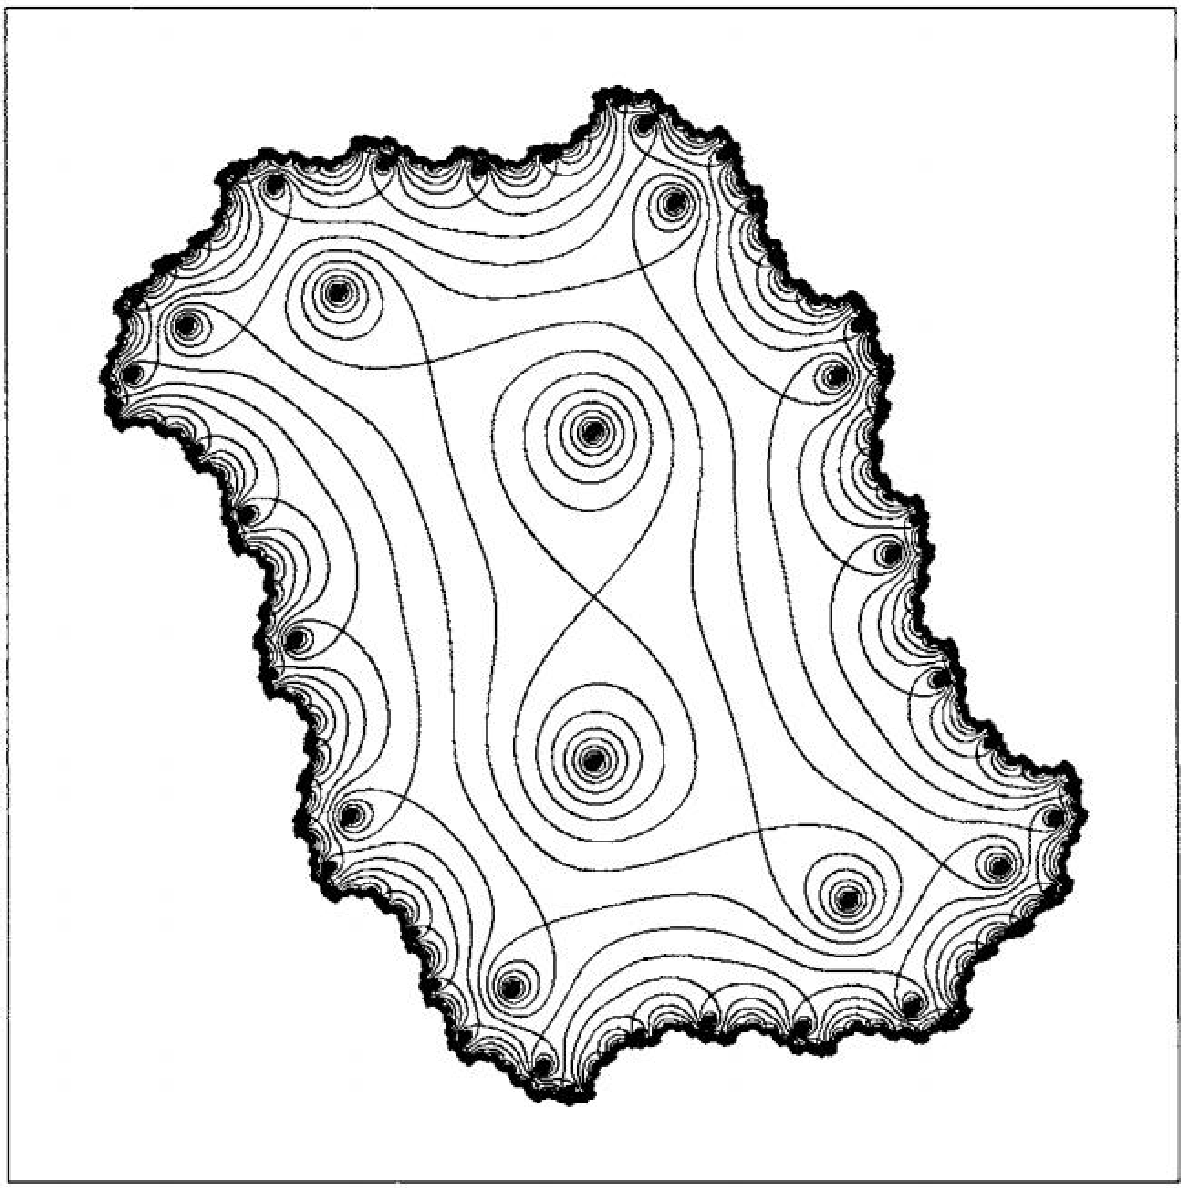
\includegraphics[width=6cm]{resources/ch-08/graph-border.pdf}
    \caption{[(Milnor 2006), p.80]Julia set for $f(z)=z^2+0.7iz$. The critical point $-0.35i$ is at the centre of the figure, and the origin is the centre of the nested circles directly above it. We see that the upper half of the figure eight bounds the region $\psi\left(\D_r\right)$ described below.}
\end{figure}
\begin{proof}
    First observe that $\linV_\eps$ is an inverse of $\linT$ in some neighbourhood of origin. As the derivative of $\linT$ at zero is 1 such local  $\linV_\eps$ exists. In addition, we have by the permanence principle that any holomorphic extension of $\linV_\eps$ is still an inverse of $\linT$ on its domain. 
    
    We now show that a finite ``maximal radius'' exists, i.e. an extension $\linV$ of $\linV_\eps$ cannot be defined on the entire complex plane: recall from the proof of Lemma~\ref{8:thm:attlinglob} that $\linT(z)=\lambda^{-n} \linT(\iter{f}{n}(z))$, so $\iter{f}{n}\left(\linV(\lin{z})\right)=\linV(\lambda^n\lin{z})$. Letting $n\tendsto\infty$ we have $\linV(0)=0$, which tells us that any extension $\linV$ of $\linV_\eps$ has its codomain in the basin of attraction $\basin$. In particular, it maps any disc $\D_R$ into $\basin^0$, due to the connectedness of $\D_R$. Now suppose that $\linV$ is defined on the entire complex plane:  $\linV:\C\to\basin^0$. Now, $\basin^0$ omits more than three points from $\widehat{\C}$ hence is hyperbolic( It omits the whole Julia set which is non empty and no isolated point (Milnor 2006) and thus by Picard's theorem $\linV$ would be a constant map, which is impossible as 0 is not a critical point.
    
    Thus there exists a maximal open $\D_{r}$ on which the extension $\linV=\linV_r$ is defined. Where $U$ is the open set $\linV\left(\D_{r}\right) \subset \basin^{0}$, the following diagram commutes:
    
    \begin{equation*}
        \begin{tikzcd}
        U \ar[r, "f"] \ar[d, "\linT", shift left] & f(U) \ar[d, "\linT", shift left] \\
        \D_r \ar[u, "\linV", shift left] \ar[r, "\lambda \cdot"'] & \lambda\D_r \ar[u, "\linV", shift left]
        \end{tikzcd}
    \end{equation*}

    Next, we show that the image of the boundary of the maximal domain $\D_r$ must contain a critical point.
    We prove this by contradiction, assume there is no critical point on the image of the boundary of the maximal domain $\D_r$.
    We have $f(\cl{U})\subset\cl{f(U)}=\cl{\linV\left(\D_R\right)} \subset U$,
    implying that $\cl {U}$ is mapped to $U $ under $f$. Since $U\subseteq\basin^0$, this means $\cl{U} \subseteq\basin^0$. So we have $\linT$ defined in some neighbourhood of $\cl {U}$. Differentiating $\linT(f(z))=\lambda \linT(z)$, we have $\tilde{\linT}(f(z)) f'(z)=\lambda \tilde{\linT}(z)$. Now for any $z$ which is \emph{not} a critical point, $ f'(z) \neq 0$. As $\linT$ is injective in $U$ $\tilde{\linT}(f(z))\neq 0$, $\tilde{\linT}(z)\neq 0$, thus $\linT$ has a local inverse on some open disc about $\lin{z}=\linT(z)$. The union of these discs covers the boundary of $\D_{r}$ and so by compactness of $\partial \D_{r}$ 
     , a finite union covers $\partial\D_{r}$, and thus the domain of the inverse can be extended to a strictly larger disc, contradicting maximality of $\D_{r}$.
   
    Thus there must exist at least one critical point on the boundary of image of $\D_r$.

    Finally, we construct an extension of $\linV_r$ to the boundary.
     Choosing a sequence $(\lin{z}_n)$ on $\D_r$ converging to some point $\lin{z}_\infty \in \partial \D_{R}$, we have $f(\linV_r(\lin{z}_n))=\linV_r(\lambda \lin{z}_{n}) \tendsto \linV_r\left(\lambda \lin{z}_{\infty}\right)$ as $n \tendsto \infty$. Since $\abs{\lambda}<1$, $\lambda \lin{z}_{\infty}\in\D_{r}$,  $z=\linV_r(\lambda \lin{z}_{\infty})$ is well-defined. Thus every convergent subsequence of $\linV_r (\lin{z}_{n})$ converges to some point in the finite set $f\inv\left(\{z\}\right)$, and the set of limit points of $\linV(\lin{z})$ as $\lin{z} \tendsto \lin{z}_{\infty}$ is a subset of $f\inv\left(\left\{z\right\}\right)$ by the argument above. Since the set of limit points of $\linV(\lin{z})$ as $\lin{z} \tendsto \lin{z}_{\infty}$ is connected(Consider any two points in this set $\linV(\lin{z}_{1_\infty})$ and $\linV(\lin{z}_{2_\infty})$ where $\lin{z}_{1_{n}} \rightarrow  \lin{z}_{1_\infty}$ , $\lin{z}_{2_{n}} \rightarrow  \lin{z}_{2_\infty}$. Then consider the image of the line segment $S_{n}$ joining $\lin{z}_{1_{n}}$ and $\lin{z}_{2_{n}}$ under $\linV$ and this is connected  So if we let $n\rightarrow \infty$ we see $\linV(S_{\infty})$ is connected and contain $\linV(\lin{z}_{1_\infty})$ and $\linV(\lin{z}_{2_\infty})$. As this is true for any two points in this set the whole set is connected) ,
    it contains exactly one element, namely $z_{0}$. Thus any convergent sequence $\linV_r(\lin{z}_n)$ converges to the same limit for any sequence $\lin{z}_{n} \to \lin{z}_{\infty}$. Thus this extension $\linV_r(\lin{z}_{\infty})=z_{0}$ is continuous.
\end{proof} 

\subsection{Attracting Periodic Orbits}

\begin{dfn}
    A \emph{periodic orbit} is an orbit $z_0 \rightarrow z_1 \rightarrow z_2 \rightarrow \cdots $ such that $z_m =\iter{f}{m}(z_0)=z_0$ for some integer $m$. A periodic orbit is called \emph{attracting} if the derivative $\abs{\left(\iter{f}{m}\right)'\left(z_{k}\right)}<1$. 
    
    (Note that in the complex plane, this derivative is equal, by the chain rule, to $ \prod f'(z_k)$ thus is same for all $z_i$. This independence of $z_i$ is also true on Riemann sphere.)
\end{dfn}

A periodic orbit can be viewed as a generalisation of the notion of a fixed point: a periodic point of $f$ of period $m$ is a fixed point of the iterate $\iter{f}{m}$. Accordingly we define the immediate basin of a periodic orbit; intuitively, this captures the notion of points which asymptotically 'wrap around' the periodic orbit:

\begin{dfn}
    \label{8:dfn:orbbasin}
    Since each $z_k$ is a fixed point of $\iter{f}{m}$, they have corresponding immediate basins. The immediate basin $\basin^0(f, \mathcal{O})$ of a periodic orbit $\mathcal{O}$ is the union of the immediate basins of each point in the orbit under $\iter{f}{m}$.
\end{dfn}

\begin{thm}
    \label{8:thm:orbcrit} 
    For $f$ a nonlinear rational map, the immediate basin of every attracting periodic orbit contains at least one critical point.
\end{thm}

\begin {proof}
Clearly, $f\left(\basin^{0}\left(z_{j}\right)\right) \subset \basin^{0}\left(z_{j+1}\right)$ (any point that goes arbitrarily close to $z_j$ will be close to $z_{j+1}$ after one iterate). Inductively applying $f$, we have that $\iter{f}{m}$ will map each $\basin^{0}\left(z_{j}\right)$ into itself. 

Suppose there is no critical point in $\basin^{0}(f, \mathcal{O})$, i.e. no critical point in any of $\basin^{0}\left(z_{j}\right)$. By chain rule, this means that there is no critical point of $\iter{f}{m}$ in any of  $\basin^{0}\left(z_{j}\right)$. 

However, this is easily seen to be false: consider some point $z_j\in\mathcal{O}$. As the orbit is attracting, this point is attracting with respect to $\iter{f}{m}$. If it is super-attracting, it is itself a critical point, and if it is geometrically attracting, there is a critical point in $\basin^{0}(z_j)$ by Lemma~\ref{8:lem:inv}. Thus we must have a critical point in $\basin^{0}(f, \mathcal{O})$.
\end{proof}

\begin{cor}
    \label{8:cor:orbfin}
    Such a rational map $f$ has only finitely many attracting periodic orbits.
\end{cor}

\begin {proof}
    Since the immediate basin of different attracting periodic orbits are clearly disjoint and $f$ can have only finitely many critical points, the result follows.
\end{proof}
\begin{rmk}
    \label{8:rmk:uful}
    Theorem~\ref{8:thm:orbcrit} is useful in approximating the periodic orbits of a rational map, as one may first locate all critical points of the function and iteratively apply the function from the critical point and observe if it converges to a periodic orbit. However, this algorithm may be invalid for orbits with large periods (such as the map $f(z)=z^{2}-1.5$ for example).
\end{rmk}

\subsection{Repelling Fixed Points}
We now consider repelling points: those points with multiplier $\abs{\lambda}>1$. 

\begin{dfn}
    \label{8:dfn:rep}
    The fixed point $\fix$ of $f$ is called \emph{topologically repelling} if for some neighbourhood $\nhd$ of $\fix$, $\forall z \in \nhd $ and $z \neq \fix,\; \exists\, n \in \N$ s.t. $\iter{f}{n}\left(z\right)$ leaves $\nhd$. Thus the only orbit that stays in $\nhd$ is the orbit of the fixed point $\fix$. Here we call $\nhd$ a \emph{forward isolating neighbourhood} of $\fix$.
\end{dfn}

For holomorphic maps on the complex plane, we have a similar result to Lemma~\ref{8:lem:att}.

\begin{lem}
    \label{8:lem:rep}
    The fixed point $0$ of $ f(z)=\lambda z+a_{2} z^{2}+a_{3} z^{3}+\dots$ is topologically repelling if and only if its multiplier satisfies $\abs{\lambda}>1$.
\end{lem}

\begin{proof}
    As in Eq.~\ref{8:eq:f}, we have $f(z)=\lambda z + O(z^2)$ so there exist constants $r>0$, $C>0$ such that $\forall$ $\abs{z}<r$,
    \begin{equation*}
        \abs{f(z)-\lambda z} \leq C\abs{z^{2}}.
    \end{equation*}
     If we take $0 < r_{0} \leq r$ sufficiently small so that $c := \abs{\lambda} - Cr_{0} > 1$ and set $\nhd = \D_{r_{0}}$, then $\forall\, z \in \nhd$,
     \[
    \abs{f(z)} \geq\abs{\lambda z}-C\abs{z^{2}} = c\abs{z}
     \]
     \[
    \Longrightarrow \abs{\iter{f}{n}(z)} \geq c^{n}\abs{z}.
    \]
    As, the $RHS$ of the final inequality $\tendsto \infty$ as $n \tendsto \infty, \forall z \in \nhd \minuset \{0\}$ since $c > 1$. Thus, $\exists\; n>0$ s.t. $f^{\circ n}(z)$ will $\nhd$ for $z\ne 0$, as required.

    Conversely, suppose $\hat{p}$ is topologically repelling fixed point of $f$. Then certainly $\hat{p}$ is \emph{not} topologically attracting and so by Lemma~\ref{8:lem:att}, $\lambda = f^{\prime}(\hat{p}) \neq 0$. Thus, by the Inverse Function Theorem, we can choose some compact forward isolating neighbourhood $\nhd$ of $\hat{p}$ which $f$ maps homeomorphically onto a compact neighbourhood $f(\nhd)$. Define
    \begin{equation*}
        \nhd^k=N \cap f\inv(\nhd) \cap \iter{(f\inv)}{2}(\nhd)\cap \dots \cap \iter{(f\inv)}{k}(\nhd)
    \end{equation*}
    So we have $\nhd \supset \nhd^1 \supset \nhd^2 \supset \dots$ is a nested sequence of compact sets all containing $\hat{p}$. Since $\hat{p}$ is topologically repelling, the intersection of these nested sets contains only the fixed point thus its diameter tends to 0. 
    
    From our construction, we immediately have $f(\nhd^k) = \nhd^{k-1} \cap f(\nhd)$ and observing that $\nhd^k\subseteq f(\nhd)$ for sufficiently large $k$ (because the diameter of $\nhd^k$ tends to 0),
     we have $f(\nhd^k) = \nhd^{k-1}$ for suffiently large $k$. If $\nhd_0^k$ denotes the connected component of $\hat{p}$ in $\nhd^k$, we see that $f\inv$ maps $\nhd_0^{k-1}$ biholomorphically onto the strictly smaller set $\nhd_0^k$. By Schwarz's lemma, the multiplier of $f\inv$ is $<1 \Longrightarrow \abs{\lambda^{-1}} < 1 \Longrightarrow \abs{\lambda} > 1$. 
\end{proof}

One may imagine that the global linearisation in the repelling case is similar to that in the attracting case. However, there isn't really such a thing as a ``repelling basin'' -- instead we can generalise $\linV_\eps$ to the entire complex plane. Here we consider $f : \C \rightarrow \C$.

\begin{thm}
    \label{8:thm:replinglob}
    For a repelling fixed point of $f$, there exists an entire bijective function $\linV$ such that $\linV (0)=0$ and $\linV$ conjugates $f$ to the linear map $\lin{z} \mapsto \lambda\lin{z}$. Moreover, $\linV$ is unique (up to multiplication by a non-zero constant).
    \begin{equation*}
        \begin{tikzcd}
            \C \ar[r, "f"] & \C \\
            \C \ar[u, "\linV"]
            \ar[r, "\lambda"'] & 
            \C \ar[u, "\linV"] \\
        \end{tikzcd}
    \end{equation*}
\end{thm} 

\begin{proof}
    Recall from theorem~\ref{8:thm:lin}, we have existence of $\linT$  and as 0 is not a critical point we have from the inverse function theorem that on some neighbourhood $\D_{\eps}(0)$, there exists a unique inverse $\linV_\eps$ with $\linV_{\eps}(0)=0$. 
    
    Let $z\in\C$, and choose the smallest $n$  such that $z/{\lambda ^{n}}\in\D_{\eps}(0)$, then define $\linV(z)=\iter{f}{n}(\linV_{\eps} (z/{\lambda ^{n}}))$ and the required properties and uniqueness can be verified as in Lemma~\ref{8:lem:inv}.
\end{proof}
\end{document}